\documentclass[pdftex,12pt,letter]{article}
\usepackage[margin=0.75in]{geometry}
\usepackage{verbatim}
\usepackage{graphicx}
\usepackage{xspace}
\usepackage{cite}
\usepackage{url}
\usepackage[pdftex,pdfpagelabels,bookmarks,hyperindex,hyperfigures]{hyperref}

%\newcommand{\pd}{protoDUNE\xspace}
%\newcommand{\pdsp}{pD/SP\xspace}
\newcommand{\xrd}{XRootD\xspace}
\newcommand{\expname}{\textit{NP04}\xspace}

\title{The clustered storage option for the protoDUNE \expname Online Buffer}
\date{\today}
\author{N. Benekos, M. Potekhin and B. Viren}


\begin{document}
\maketitle

\begin{abstract}
\noindent  This note describes the clustered storage
solution for the online buffer for the CERN experiment \expname which includes the single-phase protoDUNE LArTPC detector.
Basic data characteristics and  parameters of such storage are estimated. \xrd is proposed as the underlying
storage clustering technology. It is suggested that a portion of the existing   \textit{Neutrino Platform}
computer cluster at CERN (``\texttt{neut}'') be utilized for the development, testing and actual implementation of the \expname online buffer. 
\end{abstract}

%%%%%%%%%%%%%
\section{Overview}
\subsection{The Role of the Online Buffer}
\label{sec:the_role}
The online buffer of the \expname experiment must be put in place to absorb the high instantaneous (in-spill) DAQ
data rate before transmission of raw data to mass storage. It is also needed to satisfy the nominal CERN requirement of
providing 3 days worth of storage to make operation of the experiment possible in case of a network and/or central services
outage. Combined with the projected data rate, this requirement determines the overall capacity of the buffer. From the buffer,
the data needs to be delivered to the high-performance  disk storage (EOS) located at the CERN central services.
The place of the buffer in the data transmission chain therefore can be visualized as in Fig.\,\ref{fig:big-picture}.
EOS serves as the staging area for data transfer to other mass storage facilities such as dCache and tape at FNAL.
\begin{figure}[tbh]
  \centering
  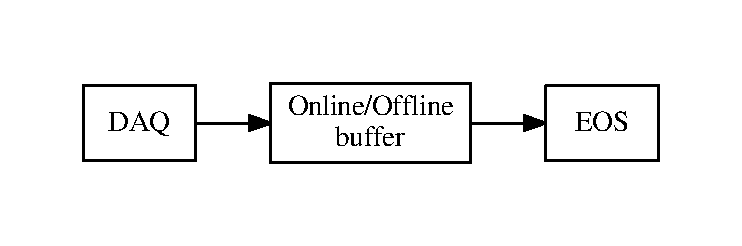
\includegraphics[width=0.7\textwidth]{figures/big-picture.pdf}
  \caption{Place of the buffer in the data transmission chain for \expname.}
  \label{fig:big-picture}
\end{figure}

\subsection{Data Characteristics}

Current estimates \cite{docdb1086} for data rate and volume bracket a range expected
in \expname \cite{docdb186} when considering in-spill beam triggers and out-of-spill cosmic ray muon triggers.
Three scenarios are considered.  The two that bracket the range are named ``Central'' and ``High rate''.  
Critical assumptions are listed below:
\begin{itemize}
\item beam spill is 4.5 seconds and cycle is 22.5 seconds
\item the beam trigger rate (assumed 25 or 50 Hz)
\item one out-of-spill cosmic trigger for every in-spill beam trigger
\item read out all APAs
\item a compression factor of 4 will be applied in the DAQ
\end{itemize}

\noindent Below is the summary of the principal data characteristics for \expname at the two ends of their estimated range:

\begin{table}[tbh]
\centering
\begin{tabular}{l l}
\hline
\textbf{Metric} & \textbf{Value} \\
\hline
\hline
trigger rate            & 25 -- 50 Hz \\  \hline
peak data rate          & 1.5 -- 3.0 GB/s \\ \hline
daily data volume       &  25 -- 50TB \\ \hline
3-day buffer capacity   & 150 -- 300TB \\  \hline
\hline
\end{tabular}
\caption{\label{tab:data_char}Expected \expname data characteristics.}
\end{table}

\subsection{F-FTS}
\label{sec:f-fts}
Basic requirements for the buffer system to handle the \expname raw data are presented in \cite{docdb1209}.
The design which meets these requirements is outlined in \cite{docdb1212}. It leverages the
Fermi File Transfer System (F-FTS) to manage two essential transfers:
\begin{itemize}
\item from the online buffer to CERN mass disk storage (EOS)
\item from EOS to CERN tape (CASTOR) and  mass storage at FNAL and other US sites
\end{itemize}

\noindent It is foreseen that two distinct instances of F-FTS will be deployed to fill each
respective role. This is schematically illustrated in Fig.\,\ref{fig:ftsinstances} where these instances are labeled ``FTS-1'' and ``FTS-2''.
The ``SP Disk Buffer Farm'' in this diagram corresponds to the \expname online buffer.

\begin{figure}[tbh]
  \centering
  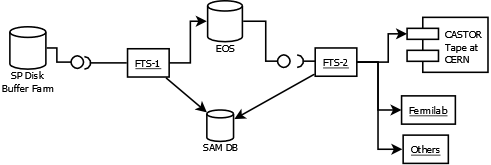
\includegraphics[width=0.7\textwidth]{figures/ftsinstances_v2.png}
  \caption{The two instances of FTS used for marshaling raw data from \expname.}
  \label{fig:ftsinstances}
\end{figure}

F-FTS uses the Fermilab SAM system for file catalog and metadata functionality,
and to keep track of the state of each transfer. 
In order to make use of this functionality, metadata
needs to be created before F-FTS takes ownership of a particular file. 
Included in this metadata is a file checksum to be used to identify any corruption during file transfer.
We seek to implement a method to calculate the checksum and collect other metadata which incurs no or minimal additional read-load on the buffer storage.  
Regardless of where the metadata are produced, the results must go into a file which will accompany the DAQ data file and be in a form suitable for consumption by F-FTS (ie, JSON format and following a prescribed schema).

F-FTS must be able to discover new files.  There are options in this
discovery process and they drive elements of the design of the buffer.
They are named by the multiplicity of FTS instances and the mechanism
of discovery:

\begin{description}
\item[1/HTTP] A single F-FTS instance is explicitly ``push''-notified
  through an HTTP POST request for each new file.  Notification is
  made by an agent running on each storage node which itself is
  triggered by an \xrd signal.
\item[1/FUSE] A single F-FTS instance polls for new files to appear in
  an \xrd-FUSE file system exported to the F-FTS host.
\item[N/local] N instances of F-FTS are run, one on each storage host.
  Each polls its local local file system for new files.
\end{description}

All options are possible and close to equivalent in terms of the
amount of required development, risk, robustness, etc.  Somewhat
subjectively, they are listed in order decreasing preference.  During
the development phase we will explore them to determine which is best
suited.

Independent from the notification mechanism, F-FTS will be responsible
for initiating the transfer of the newly buffered file from the buffer
storage to EOS.  We expect this to be done using F-FTS ``third party
transfer'' mode, specifically by invoking \xrd's direct
server-to-server transfer mechanism (eg \texttt{xrdcp --tpc}).  It is
worth noting that this transfer mechanism does not require exposing
the details of the buffer system.  All file identifiers are in a
common ``\texttt{root://}'' namespace using the host name of the
buffer system \xrd redirector.  

\section{Design of the Online Buffer}

\subsection{DAQ Assumptions}

The buffer system design relies on a few high-level assumptions about
the design of the DAQ.  In general, we assume the part of the DAQ that
``faces'' the buffer is a layer of ``Event Builder'' (EB) \textit{artDAQ}
nodes as shown schematically in Fig.~\ref{fig:upstream}.

\begin{figure}[tbh]
  \centering
  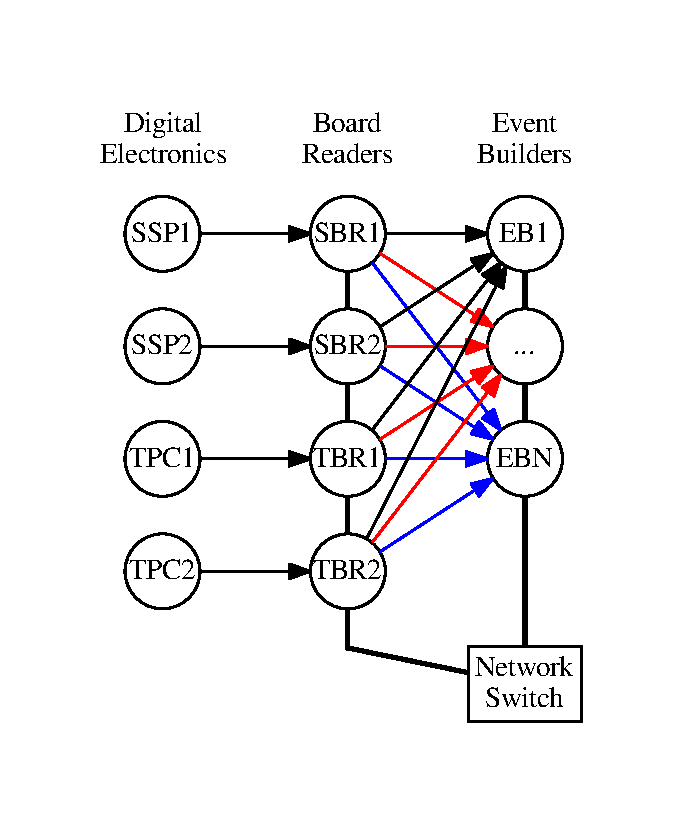
\includegraphics[width=0.5\textwidth]{figures/upstream.pdf}
  \caption{Conceptual diagram of the assumed data flow within DAQ, from the detector to the Event Builders (EB).  The buffer system depends on high level assumptions about the output of the EB layer.}
  \label{fig:upstream}
\end{figure}

We assume each EB will interact with the buffer following these steps:

\begin{enumerate}
\item EB opens an \xrd connection to the global redirector for each ``file'' using a ``\texttt{root://}'' URL that matches an prescribed prefix.
\item \xrd redirects the EB to a storage node (this is done transparently by the \xrd client library code).
\item EB streams data for some length of time.
\item EB closes the stream so that approximately 2-5~GB is transferred.
\end{enumerate}

If the EB nodes take responsibility for producing the metadata file
then it is preferred that this file is also transferred in the same
manner.  If required, mounting \xrd via FUSE on the EB nodes can be
investigated.

The network connectivity between the EB and buffer nodes still must be
worked out.  Some issues regarding this are described below, but the
exact connectivity is still to be determined.


\subsection{Attached vs Clustered Storage}
Any data taking scenario currently under consideration requires sustained rate
of ``data to disk'' in hundreds of MB per second. In practice this means that
multiple hard drives are needed to absorb such rate and have enough headroom
for stable operation of the system.
There are a few principal options for the placement of storage in the system:
\begin{itemize}
\item SAN (block-level network storage)
\item HDDs attached direectly to each of the Event Builders
\item File-level clustered storage
\end{itemize}

\noindent The SAN option has investigated and rejected for a number of reasons such as difficulty of sharing among multiple
nodes, potential for network bottlenecks etc. The attached storage option is more attractive because of its simplicity and because it
naturally leverages the parallelism of multiple Event Builders.
% and offers transparency for the DAQ developers since it is just a local file system.
However, it also has disadvantages:
\begin{itemize}
\item An F-FTS instance would need to run on each EB host which adds configuration complexity.
\item The direct association between one EB and its disks removes the ability to load balance the storage.
\item The EB hosts must directly communicate with central CERN services (EOS, in particular).
\item Failures in the buffering functionality added to an EB node directly leads to impact on the DAQ as a whole.
\end{itemize}

To counter these problems and to provide the following
benefits we will pursue a decoupled, file-level clustered storage
design based on \xrd\cite{xrootd}.  

\subsection{\xrd Storage Cluster}

The buffer will be provided as an \xrd storage cluster. With the
current rate estimations it will require the following components:

\begin{itemize}
\item Approximately 50 host computers, each with one Gbps NIC and two 3 TB HDD.
\item Network switch sufficient to connect the nodes with the DAQ LAN
  and the greater CERN network (discussed more below).
\end{itemize}

% rates, and prove it all hangs together
\noindent Under the ``High rate'' scenario the data rate during the
spill be 0.5 Gbps into each of the 50 hosts and 30 MByte/sec into each
HDD.  We assume each HDD can accept a sustained writing rate of
50~MByte/sec.  During the off-spill time, the cosmic muon trigger
produces about 0.2 Gbps into each host.  Over the entire beam cycle,
each host will receive about 540 MB.  If we assume this is read back
(in order to transfer to EOS) only during the off-spill time it
represents a 0.25~Gbps flow from HDD to network.  We expect this read
to coexist with the contemporaneous write of cosmic data.

% software stuff:
All host computers in the cluster are effectively identical in terms
of hardware, operating system and available software.  One node will
be given special configuration.  Instead of providing clustered
storage it will run the \xrd ``redirector'' as well as the instance of
F-FTS.

This design counters the problems with the alternatives that were
addressed above and it provides these additional benefits:

\begin{itemize}
\item Files are identified and located under a single namespace when
  accessed through the \xrd redirector.  Communicating an \xrd
  ``\texttt{root://} URL to the DAQ team is to a large extent the only
  ``interface'' between DAQ and this buffer system.  Similarly,
  operations by F-FTS need not be aware of any of the complexity of
  internal storage units.
\item Storage balancing and robustness against disk or host failure is
  ensured by \xrd.  A lost element does not render the buffer useless.
  Even if the redirector is lost, a storage node can be reconfigured
  to take on the task.
\item The \xrd event handling feature will be exploited to implement
  the ``push'' notification of F-FTS describe above.  It may also be
  used to execute the metadata file production process (if this task
  is not handled by the EB).
\end{itemize}

\subsection{An Extra Layer}

As described above, this design requires and extra ``layer'' of 50
hosts compared to the ``Attached storage'' option.  The cost of this
extra layer is not as high as it may first seem and it brings some
useful benefits:

\begin{itemize}
\item We plan leverage the existing ``\texttt{neut}'' cluster
  (described more below) which provides hosts with specifications that
  almost match requirements.  Initially, they lacked sufficient HDD
  capacity but plans exist to provide the required upgrades.
\item \xrd CPU requirements are almost negligible leaving a large
  fraction of the cluster available.  This ``free'' excess CPU
  capacity serves as a contingency against unexpected or ad-hoc
  processing needs.
\item Defining the boundary of this subsystem at the network allows
  for development and debugging which is decoupled from DAQ and to
  some extent F-FTS.
\item The overall design is simpler and requires less custom
  development than the ``Attached'' solution.
\item The design is based on Free Software and commodity hardware both
  of which is well understood in the community.

\item Because of the overall size of the  ``\texttt{neut}'' cluster (of over 300 nodes)
we expect to have an adquate number of potential spares at any given time.

\end{itemize}

\subsection{1\,Gbps vs 10\,Gbps}

A crucial decision in the design is the bandwidth of the storage
hosts.  The two reasonable extremes are 1 vs 10 Gbps.  The arguments
for 1 Gbps and against 10 Gbps are:

\begin{itemize}
\item 1 Gbps NIC is commodity, 10 Gbps is certainly available but not
  common.
\item 10 Gbps implies $\times 10$ more HDD in each box and the
  supporting components (hardware array, more RAM).  This is tempered
  by requiring only $\sim 5$ hosts.
\item Concentrating into fewer hosts means the system is more degraded
  by the loss of any one host.
\item \xrd has very low CPU requirements, and even at the scale of 5
  hosts, many cores will be left idle and available, but still fewer
  than in the 50 host case.
\item Maybe most importantly, we have now in hand 50 nodes from the
  ``\textbf{neut}'' cluster which has in total $\sim 350$ nodes which
  potentially can serve as spares.  These all have 1 Gbps and 2 HDD
  bays.
\end{itemize}

Entertaining the 10 Gbps option will require a cost estimate to be
performed.  The systems must likely be bought new and would number 5
to cover the scaling plus one more as a spare (live or cold) backup.
An additional low-spec host is needed to house the \xrd redirector and
F-FTS instance (under the ``1/FUSE'' or ``1/HTTP'' designs). Each
system would require $\sim 20 \times 3$ TB disks using an bus that can
assure the 50 MB/s I/O bandwidth assumption.  Of course, the systems
would require (at least) 10 Gbps NIC and a matching switch.

% \noindent Interaction of the Event Builders with a \xrd storage cluster is schematically shown in Fig.\,\ref{fig:doob-join}.

% \begin{figure}[tbh]
%   \centering
%   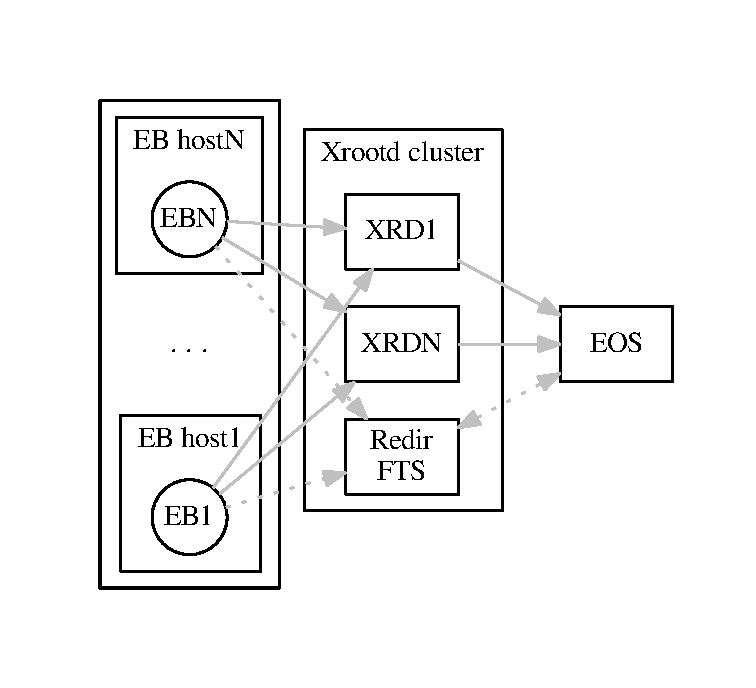
\includegraphics[width=0.5\textwidth]{figures/doob-join.pdf}
%   \caption{Conceptual diagram of the Event Builders interfacing the XRootD cluster.}
%   \label{fig:doob-join}
% \end{figure}

\section{The Cluster}
\subsection{The nodes}

The \textit{CERN Neutrino Platform} cluster (``\texttt{neut}'') is now being formed using about 350 nodes in
total reclaimed from ATLAS.  We propose to dedicate about 50 nodes in
support of developing the online buffer system for \expname.  
As described above, this is adequately scaled for storing three days worth of
data at the expected rate. To label this sub-cluster we will use the name ``\texttt{neut-spbuf}''.

Initially \texttt{neut-spbuf} will be used to implement the design
described here, perform functionality testing measure its performance
with realistic data loads.  Meanwhile, we will explore what is needed
to migrate \texttt{neut-spbuf} into actual operation.

\subsection{Networking}

As described above, the ``High rate'' scenario will produce 0.5\,Gbps
per storage host during the spill.  Initial testing will use a switch
with 48 1Gbps + 4 10Gbps ports which is procured by CERN.  This
reduces the number of storage nodes to 47 (with the 48th being the
\xrd redirector and F-FTS host).  During the development phase, the
4$\times$10 Gbps ports can be used to connect to the greater CERN
network, to the \expname detector or a dedicated high-rate data source
with 10+ Gbps NIC(s) (hardware for this is not yet identified).

During initial testing we will request a 20 Gbps link between the
current location of \texttt{neut}\footnote{CERN building 185} and
central CERN computing services including EOS and the \expname detector
site\footnote{CERN building EHN1}.

\subsection{Production}

For production, we expect to move the \texttt{neut-spbuf} nodes
physically near the DAQ cluster.  As described above, the exact
network connectivity with these nodes has yet to be determined.  If
the same switch is put into service, two of its 10 Gbps ports can
connect to the DAQ switch, assuming it has ports available.  The DAQ
EB and buffer layers are ``fully connected'' so it may be required
that they be connected all by a single switch.  

\section{Additional Work Items}
There are some known items that require additional thought and R\&D.
\begin{itemize}
\item Where will the ``SAM JSON'' metadata file be produced?  See
  comments in \ref{sec:f-fts} The two identified options are the Event
  Builders and the \xrd storage hosts.
\item Do we turn on \xrd-FUSE to give F-FTS a file system to poll or
  do we use HTTP POST to ``push'' notifications of new files?
\item What is the connectivity between DAQ EB and buffer nodes?  Do we
  connect DAQ switch to buffer switch?  Do we have one shared switch?
\item Will the switch still perform well when it sees 50\% saturation
  (one-way) on all its ports?
\item We must implement a ``recovery'' mode that identifies files that
  failed to transfer to EOS and attempts to remedy.
\item Some monitoring is needed to notify of any failures and indicate
  success.  Responsibility for a file starts on an \xrd
  \texttt{open()} call by the DAQ and finishes when confirmation that
  a file has been written successfully to EOS (at least).  
\end{itemize}



\begin{thebibliography}{1}
\bibitem{docdb1086}
{DUNE DocDB 1086: \textit{ protoDUNE/SP data scenarios with full stream (spreadsheet)}}\\
\url{http://docs.dunescience.org:8080/cgi-bin/ShowDocument?docid=1086}

\bibitem{docdb186}
{DUNE DocDB 186: \textit{ ProtoDUNE Proposal}}\\
\url{http://docs.dunescience.org:8080/cgi-bin/ShowDocument?docid=186}


\bibitem{docdb1209}
{DUNE DocDB 1209: \textit{Basic Requirements for the protoDUNE Raw Data Mangement System}}\\
\url{http://docs.dunescience.org:8080/cgi-bin/ShowDocument?docid=1209}


\bibitem{docdb1212}
{DUNE DocDB 1212: \textit{Design of the Data Management System for the protoDUNE Experiment}}\\
\url{http://docs.dunescience.org:8080/cgi-bin/ShowDocument?docid=1212}



\bibitem{xrootd}
{XRootD, high performance, scalable fault tolerant access to data  repositories}.\\
  \url{http://xrootd.org/}.

\end{thebibliography}


\end{document}

%%% Local Variables:
%%% mode: latex
%%% TeX-master: t
%%% End:
